\documentclass[12pt]{article}
\usepackage[utf8]{inputenc}
\usepackage{amsmath, amssymb}
\usepackage{geometry}
\usepackage{tikz, pgfplots}
\pgfplotsset{compat=1.16}
\geometry{margin=1in}

\title{The Specific-Factors Model}
\author{ECON 308 -- International Economic Relations}
\date{Fall 2025}

\begin{document}
\maketitle


Two goods: Manufactures $(M)$ and Food $(F)$. Labor is mobile across sectors. Capital $(K)$ is specific to $M$, land $(T)$ is specific to $F$. Production:
\[
Q_M = K^{1/2} L_M^{1/2}, \qquad Q_F = T^{1/2} L_F^{1/2}, \qquad L_M + L_F = L.
\]
Competitive wages equal value marginal products: $w = P_M \cdot MPL_M = P_F \cdot MPL_F$.

\bigskip

\section*{Problem 1: Production Functions and MPLs}
\textbf{(a)} Derive $MPL_M$ and $MPL_F$. \quad
\textbf{(b)} Evaluate at $K=T=100$ with $L=100$ and $L_M=L_F=50$.

\subsection*{Solution 1}
\[
MPL_M=\frac{\partial Q_M}{\partial L_M}=\tfrac12 K^{1/2} L_M^{-1/2},\qquad
MPL_F=\tfrac12 T^{1/2} L_F^{-1/2}.
\]
At $K=T=100$ and $L_M=L_F=50$,
\[
MPL_M=\frac{1}{2}\cdot 10 \cdot 50^{-1/2}\approx 0.707,\qquad
MPL_F\approx 0.707.
\]

\bigskip

\section*{Problem 2: Wage and Labor Allocation (Home)}
Let prices be $P_M=2$ and $P_F=1$. Consider \textbf{Home} with
\[
K=144,\quad T=64,\quad L=100.
\]
\textbf{(a)} State the condition for labor allocation. \quad
\textbf{(b)} Solve for $L_M, L_F$ and $w$.

\subsection*{Solution 2}
\textbf{(a)} Equalize VMPLs:
\[
P_M \cdot \tfrac12 K^{1/2} L_M^{-1/2} \;=\; P_F \cdot \tfrac12 T^{1/2} L_F^{-1/2}.
\]
\textbf{(b)} With $K^{1/2}=12$, $T^{1/2}=8$, $L_F=100-L_M$:
\[
2 \cdot \frac{12}{\sqrt{L_M}} = \frac{8}{\sqrt{100-L_M}}
\;\Rightarrow\; \frac{24}{\sqrt{L_M}}=\frac{8}{\sqrt{100-L_M}}.
\]
Squaring and solving yields $L_M=90$, $L_F=10$. Wage:
\[
w = P_M \cdot MPL_M
= 2 \cdot \frac{1}{2}\cdot \frac{12}{\sqrt{90}}
= \frac{12}{\sqrt{90}}
\approx 1.265.
\]

\bigskip

\section*{Problem 3: Price Change and Distribution (Home)}
Keep Home endowments. Increase $P_M$ to $3$ while $P_F=1$.
\begin{enumerate}
\item[(a)] Solve for the new $L_M,L_F$ and $w$.
\item[(b)] Who gains and who loses among capital owners, landowners, and workers in Home?
\end{enumerate}

\subsection*{Solution 3}
\textbf{(a)}
\[
3 \cdot \frac{12}{\sqrt{L_M}} = \frac{8}{\sqrt{100-L_M}}
\;\Rightarrow\; \frac{36}{\sqrt{L_M}}=\frac{8}{\sqrt{100-L_M}}.
\]
Square and solve:
\(
\frac{1296}{L_M}=\frac{64}{100-L_M}
\Rightarrow 1296(100-L_M)=64L_M
\Rightarrow L_M\approx 95.2,\ L_F\approx 4.8.
\)
Wage:
\[
w = 3 \cdot \tfrac12 \cdot \frac{12}{\sqrt{95.2}}
= \frac{18}{\sqrt{95.2}}
\approx 1.845.
\]
\textbf{(b)} Capital owners in $M$ gain, landowners in $F$ lose, workers see a nominal wage increase that is smaller than the proportional rise in $P_M$ but larger than in $P_F$; real wage rises in $F$ units and falls in $M$ units.

\bigskip
\newpage
\section*{Problem 3: Two Countries, Opportunity Costs, Comparative Advantage, and Trade}
Now introduce \textbf{Foreign} with endowments reversed:
\[
K^{*}=64,\quad T^{*}=144,\quad L^{*}=100.
\]
Assume the same production functions.

\begin{enumerate}
\item[(c)] Show that the marginal \emph{opportunity cost} of $M$ in units of $F$ equals the slope of the PPF in the SF model: \(
OC_M = \left.\dfrac{dQ_F}{dQ_M}\right|_{L} = \dfrac{MPL_F}{MPL_M}.
\)
\item[(d)] Compute $OC_M$ for Home and Foreign at $L_M=L_F=50$ and $L_M^{*}=L_F^{*}=50$ using your MPL formulas.
\item[(e)] Identify which country has comparative advantage in $M$ and which in $F$.
\item[(f)] Let the world relative price satisfy
\(
\frac{P_M}{P_F}=\tilde p \in \left(\frac{2}{3},\ \frac{3}{2}\right), \text{ e.g. } \tilde p=1.2.
\)
Who exports what under free trade? Explain briefly.
\end{enumerate}

\subsection*{Solution 3 (Prime): Opportunity Costs, CA, and Trade}
\textbf{(c)} Reallocate $dL_M=-dL_F$ so $dQ_M=MPL_M\,dL_M$, $dQ_F=MPL_F\,dL_F=-MPL_F\,dL_M$. Then
\[
\frac{dQ_F}{dQ_M}=\frac{-MPL_F\,dL_M}{MPL_M\,dL_M}=\frac{MPL_F}{MPL_M}.
\]
\textbf{(d)} At $L_M=L_F=50$:
\[
MPL_M = \tfrac12 K^{1/2} 50^{-1/2},\quad MPL_F = \tfrac12 T^{1/2} 50^{-1/2}.
\]
Hence $OC_M = \dfrac{MPL_F}{MPL_M} = \dfrac{T^{1/2}}{K^{1/2}}$.
\begin{itemize}
\item Home: $K^{1/2}=12,\ T^{1/2}=8 \Rightarrow OC_M^{Home}=8/12=2/3 \approx 0.667$.
\item Foreign: $(K^{*})^{1/2}=8,\ (T^{*})^{1/2}=12 \Rightarrow OC_M^{Foreign}=12/8=3/2=1.5$.
\end{itemize}
\textbf{(e)} Home has the lower opportunity cost of $M$ and thus comparative advantage in $M$. Foreign has comparative advantage in $F$.
\textbf{(f)} With $\tilde p=1.2$ satisfying $2/3<1.2<3/2$, Home exports $M$ and imports $F$, while Foreign exports $F$ and imports $M$.

\bigskip
\newpage
\section*{Problem 4: Graphical Exercise (Home)}
Draw $w_M(L_M)=P_M \cdot MPL_M(L_M)$ and $w_F(L_M)=P_F \cdot MPL_F(100-L_M)$ for Home, and mark equilibria before and after $P_M$ rises. Use parameters from Problems 2 and 3.

\subsection*{Solution 4: Graphical Representation for Home}
\begin{center}
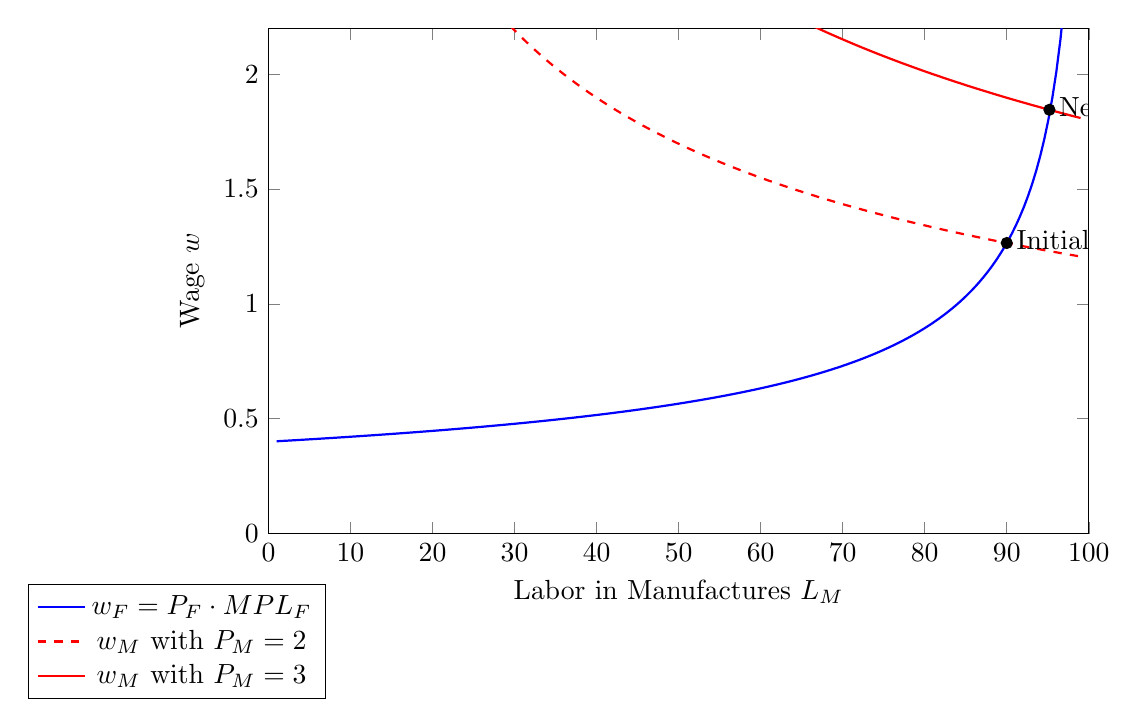
\begin{tikzpicture}
\begin{axis}[
  width=12cm, height=8cm,
  xlabel={Labor in Manufactures $L_M$},
  ylabel={Wage $w$},
  ymin=0, ymax=2.2,
  xmin=0, xmax=100,
  legend style={at={(0.07,-0.1)},anchor=north east},
  domain=1:99, samples=200
]
% Parameters: Home K^{1/2}=12, T^{1/2}=8, L=100
% Food VMPL (P_F=1): w_F = 0.5*8 / sqrt(100 - L_M) = 4 / sqrt(100 - L_M)
\addplot[thick, blue] { 4/(sqrt(100-x)) };
\addlegendentry{$w_F = P_F \cdot MPL_F$}

% Manufacturing VMPL initial (P_M=2): w_M = 2 * 0.5*12 / sqrt(L_M) = 12 / sqrt(L_M)
\addplot[thick, red, dashed] { 12/(sqrt(x)) };
\addlegendentry{$w_M$ with $P_M=2$}

% Manufacturing VMPL after price increase (P_M=3): w_M = 18 / sqrt(L_M)
\addplot[thick, red] { 18/(sqrt(x)) };
\addlegendentry{$w_M$ with $P_M=3$}

% Initial equilibrium point: L_M=90, w ≈ 1.265
\addplot[mark=*] coordinates {(90, 1.265)};
\node[anchor=west] at (axis cs:90, 1.265) {Initial eq.};

% New equilibrium point: L_M≈95.2, w ≈ 1.845
\addplot[mark=*] coordinates {(95.2, 1.845)};
\node[anchor=west] at (axis cs:95.2, 1.845) {New eq.};

\end{axis}
\end{tikzpicture}
\end{center}

\noindent
Reading the figure:
\begin{itemize}
\item Blue: $w_F(L_M)=4/\sqrt{100-L_M}$.
\item Red dashed: $w_M(L_M)=12/\sqrt{L_M}$ for $P_M=2$.
\item Red solid: $w_M(L_M)=18/\sqrt{L_M}$ for $P_M=3$.
\item Equilibrium shifts from $(L_M,w)\approx(90,\,1.265)$ to $(95.2,\,1.845)$.
\end{itemize}

\end{document}
